\documentclass[twoside]{book}

% Packages required by doxygen
\usepackage{fixltx2e}
\usepackage{calc}
\usepackage{doxygen}
\usepackage[export]{adjustbox} % also loads graphicx
\usepackage{graphicx}
\usepackage[utf8]{inputenc}
\usepackage{makeidx}
\usepackage{multicol}
\usepackage{multirow}
\PassOptionsToPackage{warn}{textcomp}
\usepackage{textcomp}
\usepackage[nointegrals]{wasysym}
\usepackage[table]{xcolor}

% Font selection
\usepackage[T1]{fontenc}
\usepackage[scaled=.90]{helvet}
\usepackage{courier}
\usepackage{amssymb}
\usepackage{sectsty}
\renewcommand{\familydefault}{\sfdefault}
\allsectionsfont{%
  \fontseries{bc}\selectfont%
  \color{darkgray}%
}
\renewcommand{\DoxyLabelFont}{%
  \fontseries{bc}\selectfont%
  \color{darkgray}%
}
\newcommand{\+}{\discretionary{\mbox{\scriptsize$\hookleftarrow$}}{}{}}

% Page & text layout
\usepackage{geometry}
\geometry{%
  a4paper,%
  top=2.5cm,%
  bottom=2.5cm,%
  left=2.5cm,%
  right=2.5cm%
}
\tolerance=750
\hfuzz=15pt
\hbadness=750
\setlength{\emergencystretch}{15pt}
\setlength{\parindent}{0cm}
\setlength{\parskip}{3ex plus 2ex minus 2ex}
\makeatletter
\renewcommand{\paragraph}{%
  \@startsection{paragraph}{4}{0ex}{-1.0ex}{1.0ex}{%
    \normalfont\normalsize\bfseries\SS@parafont%
  }%
}
\renewcommand{\subparagraph}{%
  \@startsection{subparagraph}{5}{0ex}{-1.0ex}{1.0ex}{%
    \normalfont\normalsize\bfseries\SS@subparafont%
  }%
}
\makeatother

% Headers & footers
\usepackage{fancyhdr}
\pagestyle{fancyplain}
\fancyhead[LE]{\fancyplain{}{\bfseries\thepage}}
\fancyhead[CE]{\fancyplain{}{}}
\fancyhead[RE]{\fancyplain{}{\bfseries\leftmark}}
\fancyhead[LO]{\fancyplain{}{\bfseries\rightmark}}
\fancyhead[CO]{\fancyplain{}{}}
\fancyhead[RO]{\fancyplain{}{\bfseries\thepage}}
\fancyfoot[LE]{\fancyplain{}{}}
\fancyfoot[CE]{\fancyplain{}{}}
\fancyfoot[RE]{\fancyplain{}{\bfseries\scriptsize Generated by Doxygen }}
\fancyfoot[LO]{\fancyplain{}{\bfseries\scriptsize Generated by Doxygen }}
\fancyfoot[CO]{\fancyplain{}{}}
\fancyfoot[RO]{\fancyplain{}{}}
\renewcommand{\footrulewidth}{0.4pt}
\renewcommand{\chaptermark}[1]{%
  \markboth{#1}{}%
}
\renewcommand{\sectionmark}[1]{%
  \markright{\thesection\ #1}%
}

% Indices & bibliography
\usepackage{natbib}
\usepackage[titles]{tocloft}
\setcounter{tocdepth}{3}
\setcounter{secnumdepth}{5}
\makeindex

% Hyperlinks (required, but should be loaded last)
\usepackage{ifpdf}
\ifpdf
  \usepackage[pdftex,pagebackref=true]{hyperref}
\else
  \usepackage[ps2pdf,pagebackref=true]{hyperref}
\fi
\hypersetup{%
  colorlinks=true,%
  linkcolor=blue,%
  citecolor=blue,%
  unicode%
}

% Custom commands
\newcommand{\clearemptydoublepage}{%
  \newpage{\pagestyle{empty}\cleardoublepage}%
}

\usepackage{caption}
\captionsetup{labelsep=space,justification=centering,font={bf},singlelinecheck=off,skip=4pt,position=top}

%===== C O N T E N T S =====

\begin{document}

% Titlepage & ToC
\hypersetup{pageanchor=false,
             bookmarksnumbered=true,
             pdfencoding=unicode
            }
\pagenumbering{roman}
\begin{titlepage}
\vspace*{7cm}
\begin{center}%
{\Large My Project }\\
\vspace*{1cm}
{\large Generated by Doxygen 1.8.11}\\
\end{center}
\end{titlepage}
\clearemptydoublepage
\tableofcontents
\clearemptydoublepage
\pagenumbering{arabic}
\hypersetup{pageanchor=true}

%--- Begin generated contents ---
\chapter{Class Index}
\section{Class List}
Here are the classes, structs, unions and interfaces with brief descriptions\+:\begin{DoxyCompactList}
\item\contentsline{section}{\hyperlink{structnode}{node} }{\pageref{structnode}}{}
\item\contentsline{section}{\hyperlink{structnode1}{node1} }{\pageref{structnode1}}{}
\item\contentsline{section}{\hyperlink{structnode__info}{node\+\_\+info} }{\pageref{structnode__info}}{}
\end{DoxyCompactList}

\chapter{File Index}
\section{File List}
Here is a list of all files with brief descriptions\+:\begin{DoxyCompactList}
\item\contentsline{section}{\hyperlink{Lab1_8c}{Lab1.\+c} }{\pageref{Lab1_8c}}{}
\end{DoxyCompactList}

\chapter{Class Documentation}
\hypertarget{structBucket}{}\section{Bucket Struct Reference}
\label{structBucket}\index{Bucket@{Bucket}}


Collaboration diagram for Bucket\+:
\nopagebreak
\begin{figure}[H]
\begin{center}
\leavevmode
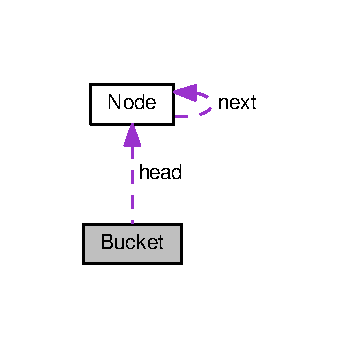
\includegraphics[width=164pt]{structBucket__coll__graph}
\end{center}
\end{figure}
\subsection*{Public Attributes}
\begin{DoxyCompactItemize}
\item 
struct \hyperlink{structNode}{Node} $\ast$ \hyperlink{structBucket_afa23129a049b6cb4ad5403a5662b938f}{head}
\end{DoxyCompactItemize}


\subsection{Member Data Documentation}
\index{Bucket@{Bucket}!head@{head}}
\index{head@{head}!Bucket@{Bucket}}
\subsubsection[{\texorpdfstring{head}{head}}]{\setlength{\rightskip}{0pt plus 5cm}struct {\bf Node}$\ast$ Bucket\+::head}\hypertarget{structBucket_afa23129a049b6cb4ad5403a5662b938f}{}\label{structBucket_afa23129a049b6cb4ad5403a5662b938f}


The documentation for this struct was generated from the following file\+:\begin{DoxyCompactItemize}
\item 
\hyperlink{BucketSort_8cpp}{Bucket\+Sort.\+cpp}\end{DoxyCompactItemize}

\hypertarget{structBucketList}{}\section{Bucket\+List Struct Reference}
\label{structBucketList}\index{Bucket\+List@{Bucket\+List}}


Collaboration diagram for Bucket\+List\+:
\nopagebreak
\begin{figure}[H]
\begin{center}
\leavevmode
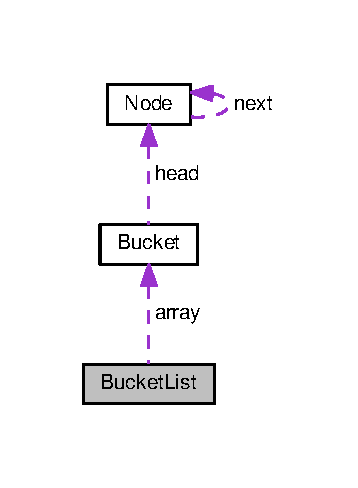
\includegraphics[width=172pt]{structBucketList__coll__graph}
\end{center}
\end{figure}
\subsection*{Public Attributes}
\begin{DoxyCompactItemize}
\item 
int \hyperlink{structBucketList_a986196d1d435700557398237ad52fee9}{V}
\item 
struct \hyperlink{structBucket}{Bucket} $\ast$ \hyperlink{structBucketList_a55c205b2d67034433e98c4e96f39095e}{array}
\end{DoxyCompactItemize}


\subsection{Member Data Documentation}
\index{Bucket\+List@{Bucket\+List}!array@{array}}
\index{array@{array}!Bucket\+List@{Bucket\+List}}
\subsubsection[{\texorpdfstring{array}{array}}]{\setlength{\rightskip}{0pt plus 5cm}struct {\bf Bucket}$\ast$ Bucket\+List\+::array}\hypertarget{structBucketList_a55c205b2d67034433e98c4e96f39095e}{}\label{structBucketList_a55c205b2d67034433e98c4e96f39095e}
\index{Bucket\+List@{Bucket\+List}!V@{V}}
\index{V@{V}!Bucket\+List@{Bucket\+List}}
\subsubsection[{\texorpdfstring{V}{V}}]{\setlength{\rightskip}{0pt plus 5cm}int Bucket\+List\+::V}\hypertarget{structBucketList_a986196d1d435700557398237ad52fee9}{}\label{structBucketList_a986196d1d435700557398237ad52fee9}


The documentation for this struct was generated from the following file\+:\begin{DoxyCompactItemize}
\item 
\hyperlink{BucketSort_8cpp}{Bucket\+Sort.\+cpp}\end{DoxyCompactItemize}

\hypertarget{structNode}{}\section{Node Struct Reference}
\label{structNode}\index{Node@{Node}}


Collaboration diagram for Node\+:
\nopagebreak
\begin{figure}[H]
\begin{center}
\leavevmode
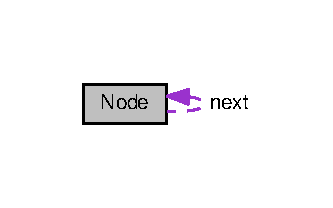
\includegraphics[width=160pt]{structNode__coll__graph}
\end{center}
\end{figure}
\subsection*{Public Attributes}
\begin{DoxyCompactItemize}
\item 
int \hyperlink{structNode_aaa0cd30d78a90c5a6ab64eb3d58b8f87}{value}
\item 
struct \hyperlink{structNode}{Node} $\ast$ \hyperlink{structNode_af67b110ca1a258b793bf69d306929b22}{next}
\end{DoxyCompactItemize}


\subsection{Member Data Documentation}
\index{Node@{Node}!next@{next}}
\index{next@{next}!Node@{Node}}
\subsubsection[{\texorpdfstring{next}{next}}]{\setlength{\rightskip}{0pt plus 5cm}struct {\bf Node}$\ast$ Node\+::next}\hypertarget{structNode_af67b110ca1a258b793bf69d306929b22}{}\label{structNode_af67b110ca1a258b793bf69d306929b22}
\index{Node@{Node}!value@{value}}
\index{value@{value}!Node@{Node}}
\subsubsection[{\texorpdfstring{value}{value}}]{\setlength{\rightskip}{0pt plus 5cm}int Node\+::value}\hypertarget{structNode_aaa0cd30d78a90c5a6ab64eb3d58b8f87}{}\label{structNode_aaa0cd30d78a90c5a6ab64eb3d58b8f87}


The documentation for this struct was generated from the following file\+:\begin{DoxyCompactItemize}
\item 
\hyperlink{BucketSort_8cpp}{Bucket\+Sort.\+cpp}\end{DoxyCompactItemize}

\chapter{File Documentation}
\hypertarget{BucketSort_8cpp}{}\section{Bucket\+Sort.\+cpp File Reference}
\label{BucketSort_8cpp}\index{Bucket\+Sort.\+cpp@{Bucket\+Sort.\+cpp}}
{\ttfamily \#include $<$iostream$>$}\\*
Include dependency graph for Bucket\+Sort.\+cpp\+:
\nopagebreak
\begin{figure}[H]
\begin{center}
\leavevmode
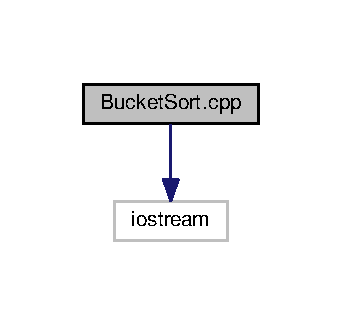
\includegraphics[width=164pt]{BucketSort_8cpp__incl}
\end{center}
\end{figure}
\subsection*{Classes}
\begin{DoxyCompactItemize}
\item 
struct \hyperlink{structNode}{Node}
\item 
struct \hyperlink{structBucket}{Bucket}
\item 
struct \hyperlink{structBucketList}{Bucket\+List}
\end{DoxyCompactItemize}
\subsection*{Functions}
\begin{DoxyCompactItemize}
\item 
struct \hyperlink{structNode}{Node} $\ast$ \hyperlink{BucketSort_8cpp_aa079f3ceaf2578ddc2fea214bac509ea}{new\+Node} (int value)
\item 
struct \hyperlink{structBucketList}{Bucket\+List} $\ast$ \hyperlink{BucketSort_8cpp_ade40d37889b230f76f75f7e7c1c44aea}{create\+Bucket} (int V)
\item 
void \hyperlink{BucketSort_8cpp_abf021c8398f9349ed3e5047ded4988f6}{add\+Node} (struct \hyperlink{structBucketList}{Bucket\+List} $\ast$bl, int bckt, int value)
\item 
void \hyperlink{BucketSort_8cpp_a8b528b158bb27fcd885205966c39cdb8}{print\+Buckets} (struct \hyperlink{structBucketList}{Bucket\+List} $\ast$bl)
\item 
int \hyperlink{BucketSort_8cpp_ae66f6b31b5ad750f1fe042a706a4e3d4}{main} ()
\end{DoxyCompactItemize}


\subsection{Function Documentation}
\index{Bucket\+Sort.\+cpp@{Bucket\+Sort.\+cpp}!add\+Node@{add\+Node}}
\index{add\+Node@{add\+Node}!Bucket\+Sort.\+cpp@{Bucket\+Sort.\+cpp}}
\subsubsection[{\texorpdfstring{add\+Node(struct Bucket\+List $\ast$bl, int bckt, int value)}{addNode(struct BucketList *bl, int bckt, int value)}}]{\setlength{\rightskip}{0pt plus 5cm}void add\+Node (
\begin{DoxyParamCaption}
\item[{struct {\bf Bucket\+List} $\ast$}]{bl, }
\item[{int}]{bckt, }
\item[{int}]{value}
\end{DoxyParamCaption}
)}\hypertarget{BucketSort_8cpp_abf021c8398f9349ed3e5047ded4988f6}{}\label{BucketSort_8cpp_abf021c8398f9349ed3e5047ded4988f6}

\begin{DoxyCode}
54 \{
55     \textcolor{comment}{// Creating new data node.}
56     \textcolor{keyword}{struct }\hyperlink{structNode}{Node} *newnode = \hyperlink{BucketSort_8cpp_aa079f3ceaf2578ddc2fea214bac509ea}{newNode}(\hyperlink{structNode_aaa0cd30d78a90c5a6ab64eb3d58b8f87}{value});
57     \textcolor{keyword}{struct }\hyperlink{structNode}{Node} *temp = \textcolor{keyword}{new} \hyperlink{structNode}{Node};
58  
59     \textcolor{keywordflow}{if}(bl->\hyperlink{structBucketList_a55c205b2d67034433e98c4e96f39095e}{array}[bckt].\hyperlink{structBucket_afa23129a049b6cb4ad5403a5662b938f}{head} != NULL)
60     \{
61         temp = bl->\hyperlink{structBucketList_a55c205b2d67034433e98c4e96f39095e}{array}[bckt].\hyperlink{structBucket_afa23129a049b6cb4ad5403a5662b938f}{head};
62  
63         \textcolor{comment}{// Sorting.}
64         \textcolor{comment}{// If the head node value is lesser than the newnode value, then add node at beginning.}
65         \textcolor{keywordflow}{if}(temp->\hyperlink{structNode_aaa0cd30d78a90c5a6ab64eb3d58b8f87}{value} > newnode->\hyperlink{structNode_aaa0cd30d78a90c5a6ab64eb3d58b8f87}{value})
66         \{
67             newnode->\hyperlink{structNode_af67b110ca1a258b793bf69d306929b22}{next} = bl->\hyperlink{structBucketList_a55c205b2d67034433e98c4e96f39095e}{array}[bckt].\hyperlink{structBucket_afa23129a049b6cb4ad5403a5662b938f}{head};
68             bl->\hyperlink{structBucketList_a55c205b2d67034433e98c4e96f39095e}{array}[bckt].\hyperlink{structBucket_afa23129a049b6cb4ad5403a5662b938f}{head} = newnode;
69         \}
70         \textcolor{keywordflow}{else}
71         \{
72             \textcolor{comment}{// Search for the node whose value is more than the newnode value.}
73             \textcolor{keywordflow}{while}(temp->\hyperlink{structNode_af67b110ca1a258b793bf69d306929b22}{next} != NULL)
74             \{
75                 \textcolor{keywordflow}{if}((temp->\hyperlink{structNode_af67b110ca1a258b793bf69d306929b22}{next})->value > newnode->\hyperlink{structNode_aaa0cd30d78a90c5a6ab64eb3d58b8f87}{value})
76                     \textcolor{keywordflow}{break};
77  
78                 temp = temp->\hyperlink{structNode_af67b110ca1a258b793bf69d306929b22}{next};
79             \}
80  
81             \textcolor{comment}{// Insert newnode after temp node.}
82             newnode->\hyperlink{structNode_af67b110ca1a258b793bf69d306929b22}{next} = temp->\hyperlink{structNode_af67b110ca1a258b793bf69d306929b22}{next};
83             temp->\hyperlink{structNode_af67b110ca1a258b793bf69d306929b22}{next} = newnode;
84         \}
85     \}
86     \textcolor{keywordflow}{else}
87     \{
88         \textcolor{comment}{// Assign head of the Bucket as newnode since bucket head is NULL.}
89         bl->\hyperlink{structBucketList_a55c205b2d67034433e98c4e96f39095e}{array}[bckt].\hyperlink{structBucket_afa23129a049b6cb4ad5403a5662b938f}{head} = newnode;
90     \}
91 \}
\end{DoxyCode}


Here is the call graph for this function\+:
\nopagebreak
\begin{figure}[H]
\begin{center}
\leavevmode
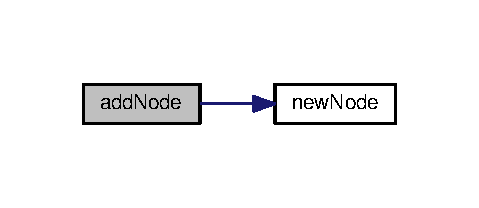
\includegraphics[width=230pt]{BucketSort_8cpp_abf021c8398f9349ed3e5047ded4988f6_cgraph}
\end{center}
\end{figure}


\index{Bucket\+Sort.\+cpp@{Bucket\+Sort.\+cpp}!create\+Bucket@{create\+Bucket}}
\index{create\+Bucket@{create\+Bucket}!Bucket\+Sort.\+cpp@{Bucket\+Sort.\+cpp}}
\subsubsection[{\texorpdfstring{create\+Bucket(int V)}{createBucket(int V)}}]{\setlength{\rightskip}{0pt plus 5cm}struct {\bf Bucket\+List}$\ast$ create\+Bucket (
\begin{DoxyParamCaption}
\item[{int}]{V}
\end{DoxyParamCaption}
)}\hypertarget{BucketSort_8cpp_ade40d37889b230f76f75f7e7c1c44aea}{}\label{BucketSort_8cpp_ade40d37889b230f76f75f7e7c1c44aea}

\begin{DoxyCode}
37 \{
38     \textcolor{keywordtype}{int} i;
39     \textcolor{keyword}{struct }\hyperlink{structBucketList}{BucketList}* bl = \textcolor{keyword}{new} \hyperlink{structBucketList}{BucketList};
40  
41     bl->\hyperlink{structBucketList_a986196d1d435700557398237ad52fee9}{V} = \hyperlink{structBucketList_a986196d1d435700557398237ad52fee9}{V};
42     bl->\hyperlink{structBucketList_a55c205b2d67034433e98c4e96f39095e}{array} = \textcolor{keyword}{new} \hyperlink{structBucket}{Bucket}[\hyperlink{structBucketList_a986196d1d435700557398237ad52fee9}{V}];   
43  
44  
45     \textcolor{comment}{// Initialize each Bucket list as empty by making head as NULL.}
46     \textcolor{keywordflow}{for}(i = 0; i < \hyperlink{structBucketList_a986196d1d435700557398237ad52fee9}{V}; i++)
47         bl->\hyperlink{structBucketList_a55c205b2d67034433e98c4e96f39095e}{array}[i].\hyperlink{structBucket_afa23129a049b6cb4ad5403a5662b938f}{head} = NULL;
48  
49     \textcolor{keywordflow}{return} bl;
50 \}
\end{DoxyCode}
\index{Bucket\+Sort.\+cpp@{Bucket\+Sort.\+cpp}!main@{main}}
\index{main@{main}!Bucket\+Sort.\+cpp@{Bucket\+Sort.\+cpp}}
\subsubsection[{\texorpdfstring{main()}{main()}}]{\setlength{\rightskip}{0pt plus 5cm}int main (
\begin{DoxyParamCaption}
{}
\end{DoxyParamCaption}
)}\hypertarget{BucketSort_8cpp_ae66f6b31b5ad750f1fe042a706a4e3d4}{}\label{BucketSort_8cpp_ae66f6b31b5ad750f1fe042a706a4e3d4}

\begin{DoxyCode}
115 \{
116     \textcolor{comment}{// Create the BucketLists for the data and set 10 as default number of Buckets.}
117     \textcolor{keywordtype}{int} \hyperlink{structBucketList_a986196d1d435700557398237ad52fee9}{V} = 10, range, NOE, i;
118     \textcolor{keyword}{struct }\hyperlink{structBucketList}{BucketList}* mybucket = \hyperlink{BucketSort_8cpp_ade40d37889b230f76f75f7e7c1c44aea}{createBucket}(V);
119  
120  
121     cout<<\textcolor{stringliteral}{"\(\backslash\)n\(\backslash\)nEnter the upper limit in the power of 10 (10 or 100 or 1000 ..) to create Bucket: "};
122     cin>>range;
123  
124     \textcolor{comment}{// Dividing range into 10 parts so it will have 10 buckets as default.}
125     range = range/10;
126  
127     cout<<\textcolor{stringliteral}{"\(\backslash\)nEnter the number of data element to be sorted: "};
128     cin>>NOE;
129     \textcolor{keywordtype}{int} arr[NOE];
130  
131     \textcolor{keywordflow}{for}(i = 0; i < NOE; i++)
132     \{
133         cout<<\textcolor{stringliteral}{"Enter element "}<<i+1<<\textcolor{stringliteral}{" : "};
134         cin>>arr[i];
135         \hyperlink{BucketSort_8cpp_abf021c8398f9349ed3e5047ded4988f6}{addNode}(mybucket, arr[i]/range, arr[i]);
136     \}
137  
138     \textcolor{comment}{// Print the adjacency list representation of the BucketList i.e the sorted Output.}
139     cout<<\textcolor{stringliteral}{"\(\backslash\)nSorted Data "};
140     \hyperlink{BucketSort_8cpp_a8b528b158bb27fcd885205966c39cdb8}{printBuckets}(mybucket);
141  
142     \textcolor{keywordflow}{return} 0;
143 \}\end{DoxyCode}


Here is the call graph for this function\+:
\nopagebreak
\begin{figure}[H]
\begin{center}
\leavevmode
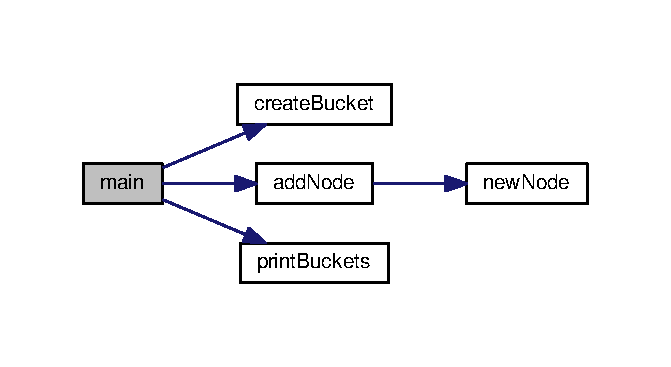
\includegraphics[width=322pt]{BucketSort_8cpp_ae66f6b31b5ad750f1fe042a706a4e3d4_cgraph}
\end{center}
\end{figure}


\index{Bucket\+Sort.\+cpp@{Bucket\+Sort.\+cpp}!new\+Node@{new\+Node}}
\index{new\+Node@{new\+Node}!Bucket\+Sort.\+cpp@{Bucket\+Sort.\+cpp}}
\subsubsection[{\texorpdfstring{new\+Node(int value)}{newNode(int value)}}]{\setlength{\rightskip}{0pt plus 5cm}struct {\bf Node}$\ast$ new\+Node (
\begin{DoxyParamCaption}
\item[{int}]{value}
\end{DoxyParamCaption}
)}\hypertarget{BucketSort_8cpp_aa079f3ceaf2578ddc2fea214bac509ea}{}\label{BucketSort_8cpp_aa079f3ceaf2578ddc2fea214bac509ea}

\begin{DoxyCode}
28 \{
29     \textcolor{keyword}{struct }\hyperlink{structNode}{Node}* newnode = \textcolor{keyword}{new} \hyperlink{structNode}{Node};
30     newnode->\hyperlink{structNode_aaa0cd30d78a90c5a6ab64eb3d58b8f87}{value} = \hyperlink{structNode_aaa0cd30d78a90c5a6ab64eb3d58b8f87}{value};
31     newnode->\hyperlink{structNode_af67b110ca1a258b793bf69d306929b22}{next} = NULL;
32     \textcolor{keywordflow}{return} newnode;
33 \}
\end{DoxyCode}
\index{Bucket\+Sort.\+cpp@{Bucket\+Sort.\+cpp}!print\+Buckets@{print\+Buckets}}
\index{print\+Buckets@{print\+Buckets}!Bucket\+Sort.\+cpp@{Bucket\+Sort.\+cpp}}
\subsubsection[{\texorpdfstring{print\+Buckets(struct Bucket\+List $\ast$bl)}{printBuckets(struct BucketList *bl)}}]{\setlength{\rightskip}{0pt plus 5cm}void print\+Buckets (
\begin{DoxyParamCaption}
\item[{struct {\bf Bucket\+List} $\ast$}]{bl}
\end{DoxyParamCaption}
)}\hypertarget{BucketSort_8cpp_a8b528b158bb27fcd885205966c39cdb8}{}\label{BucketSort_8cpp_a8b528b158bb27fcd885205966c39cdb8}

\begin{DoxyCode}
95 \{
96     \textcolor{keywordtype}{int} v;
97     \textcolor{keyword}{struct }\hyperlink{structNode}{Node}* pCrawl = \textcolor{keyword}{new} \hyperlink{structNode}{Node};
98  
99     \textcolor{keywordflow}{for}(v = 0; v < bl->\hyperlink{structBucketList_a986196d1d435700557398237ad52fee9}{V}; v++)
100     \{
101         \textcolor{comment}{// To view the data in individual bucket remove next line from comment.}
102         \textcolor{comment}{// cout<<"\(\backslash\)n\(\backslash\)t bucket "<<v+1;}
103  
104         pCrawl = bl->\hyperlink{structBucketList_a55c205b2d67034433e98c4e96f39095e}{array}[v].\hyperlink{structBucket_afa23129a049b6cb4ad5403a5662b938f}{head};
105         \textcolor{keywordflow}{while} (pCrawl != NULL)
106         \{
107             cout<<\textcolor{stringliteral}{"->"}<< pCrawl->\hyperlink{structNode_aaa0cd30d78a90c5a6ab64eb3d58b8f87}{value};
108             pCrawl = pCrawl->\hyperlink{structNode_af67b110ca1a258b793bf69d306929b22}{next};
109         \}
110     \}
111 \}
\end{DoxyCode}

%--- End generated contents ---

% Index
\backmatter
\newpage
\phantomsection
\clearemptydoublepage
\addcontentsline{toc}{chapter}{Index}
\printindex

\end{document}
